% !TeX program = pdflatex
\documentclass[tikz,border=8pt]{standalone}
\usepackage{pgfplots}
\pgfplotsset{compat=1.16}
\definecolor{FigureBlue}{HTML}{2563EB}
\definecolor{FigureOrange}{HTML}{EA580C}
\definecolor{FigureSlate}{HTML}{475569}
\begin{document}
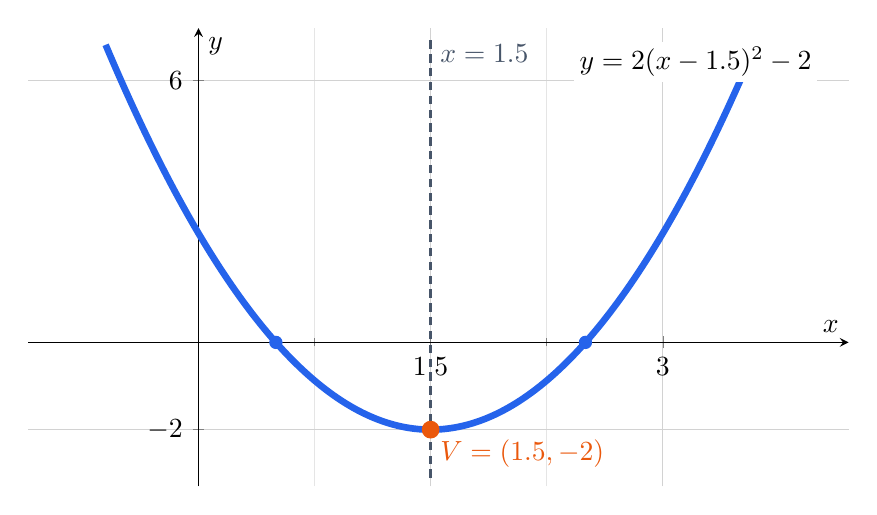
\begin{tikzpicture}
  \begin{axis}[
    width=12cm,height=7.4cm,axis lines=middle,
    xmin=-1.1,xmax=4.2,ymin=-3.3,ymax=7.2,
    xlabel={$x$},ylabel={$y$},xtick={0,1.5,3},ytick={-2,0,6},
    grid=both,minor tick num=1,clip=false,
    grid style={draw=gray!20},major grid style={draw=gray!35},
  ]
    \addplot[FigureBlue,line width=2.4pt,domain=-0.6:3.6,samples=161]
      {2*(x-1.5)^2-2};
    \draw[FigureSlate,densely dashed,line width=1.1pt]
      (axis cs:1.5,-3.1)--(axis cs:1.5,7);
    \addplot[only marks,mark=*,mark size=3pt,FigureOrange]
      coordinates {(1.5,-2)};
    \addplot[only marks,mark=*,mark size=2.2pt,FigureBlue]
      coordinates {(0.5,0) (2.5,0)};
    \node[anchor=north west,text=FigureOrange] at (axis cs:1.5,-2) {$V=(1.5,-2)$};
    \node[anchor=south west,text=FigureSlate] at (axis cs:1.5,6.2) {$x=1.5$};
    \node[anchor=north east,fill=white,inner sep=2pt] at (axis cs:4,6.9)
      {$y=2(x-1.5)^2-2$};
  \end{axis}
\end{tikzpicture}
\end{document}
